\documentclass[makesolutionspdf]{esg8022pset}
\begin{preamble}
\usepackage{amsmath}
\usepackage{amssymb}
\usepackage{enumerate}
\usepackage{graphicx}
\usepackage{hyperref}
\usepackage{mathtools}
\usepackage[per-mode=symbol]{siunitx} %If this line is giving you trouble, try replacing per-mode with per
%use inter-unit-separator={}\cdot{} ?
\providecommand{\uvec}[1]{{\hat{\bf{#1}}}}
\usepackage{pgf,tikz}
\usetikzlibrary{arrows}
\usepackage{wasysym}
\usepackage{subfig}
\makeatletter
\newcommand{\interitemtext}[1]{%
  \begin{list}{}
   {\itemindent=0mm\labelsep=0mm
   \labelwidth=0mm\leftmargin=0mm
   \addtolength{\leftmargin}{-\@totalleftmargin}}
    \item #1
  \end{list}
}
\makeatother
\renewcommand{\d}{\,d}
\providecommand{\norm}[1]{\lVert#1\rVert}

\newcommand{\Kgrad}{\left(\hat{x} \frac{\partial}{\partial x} + \hat{y} \frac{\partial}{\partial y} + \hat{z} \frac{\partial}{\partial z}\right)}
\newcommand{\Kdiv}[6]{{#4}\left(\frac{\partial {#1}}{\partial x} {#5} \frac{\partial {#2}}{\partial y} {#6}\frac{\partial #3}{\partial z} \right)}
\newcommand{\KKdiv}[6]{{#4}\left(\frac{\partial}{\partial x}{#1} {#5} \frac{\partial}{\partial y}{#2} {#6}\frac{\partial}{\partial z}{#3} \right)}
\newcommand{\dx}{\frac{\partial}{\partial x}}
\newcommand{\dy}{\frac{\partial}{\partial y}}
\newcommand{\dz}{\frac{\partial}{\partial z}}
\newcommand{\dtheta}{\frac{\partial}{\partial \theta}}
\newcommand{\dr}{\frac{\partial}{\partial r}}

\AtBeginDocument{%
  % Appologies to any future editor on the inconsistencies in TeX code and the unnecessary braces.  I'm aggregating previously typeset problems, and didn't think it worth my time to improve the quality of TeX code in ways that won't make any difference to the typeset material. -Jason Gross (jgross@mit.edu)
}%
\end{preamble}

\classname{Physics 8.022}
\semester{Spring 2011}
\problemsetnumber{8} %Put the problem set number here
\duedate{Sunday, April 3rd at 9 \textsc{pm}}
%\readingassignment{Kleppner and Kolenkow, \emph{An Introduction to Mechanics}, Chapters Seven and Eight}
\problemsettitle{Amp\`{e}re's law, Biot-Savart law}

\begin{document}

\begin{problem}{Long flat conductor}
  A long flat conductor of width $a$ carries a sheet of current $i$ (see
  \autoref{fig:flat}). You are asked to find the magnetic field (direction and
  magnitude) near the center of its flat side and and very close to the
  surface, such that the distance $R$ from the sheet is $R \ll a$.

  \begin{figure}[ht]
    \centering
    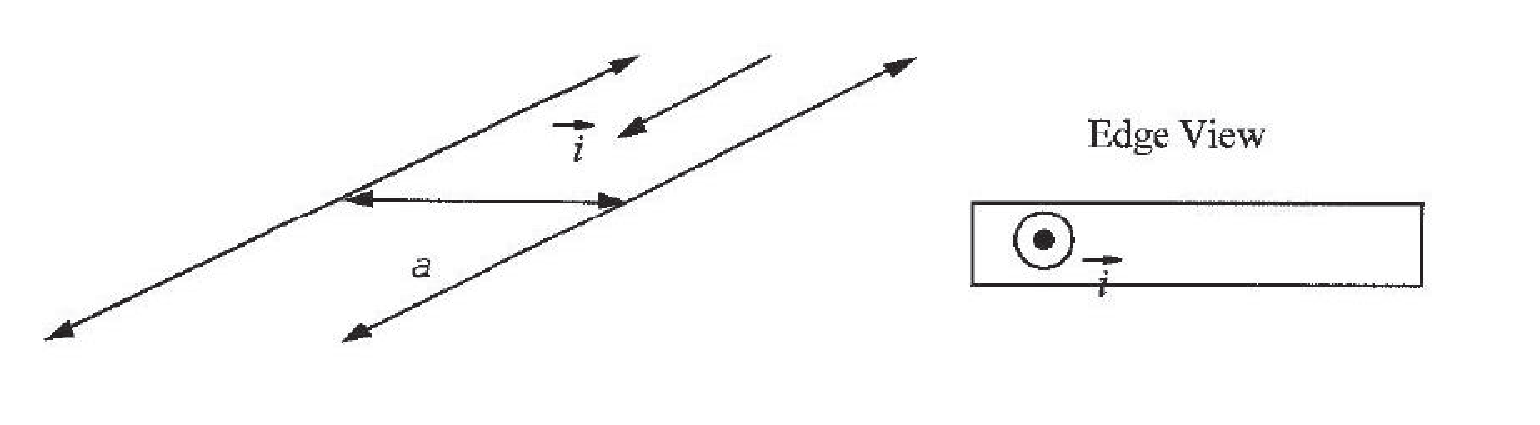
\includegraphics[width = 10cm]{flat_conductor}
    \caption{Flat conductor}
    \label{fig:flat}
  \end{figure}

\end{problem}

\begin{solution}

  \begin{figure}[ht]
    \centering
    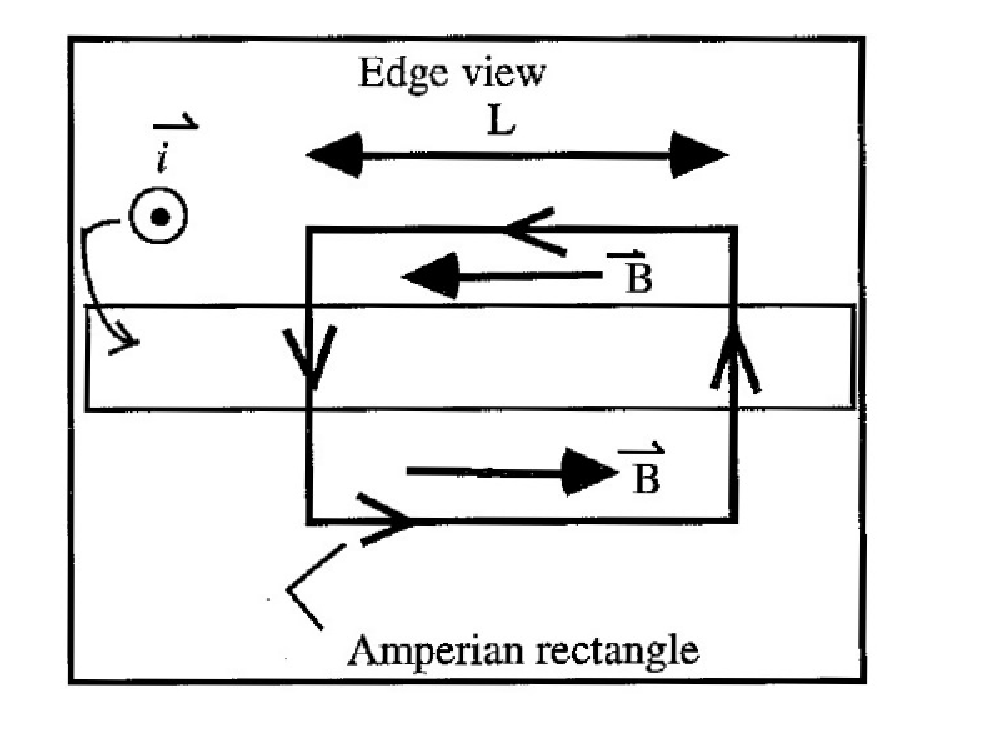
\includegraphics[width = 10cm]{flat_conductor_sol}
    \label{fig:flatsol}
  \end{figure}

  As shown in the figure, above the conductor, $\vec{B}$ points to the left,
  below the conductor, $\vec{B}$  points to the right (the current is pointing
  out of the paper).  Choose an amperian path shown in the plot, since the
  distance $R$ is much smaller than $a$, we have:
  \begin{equation}
    2B \times L = \frac{4 \pi}{c} I_{\text{enc}} = \frac{4 \pi}{c} \frac{L i}{a}
  \end{equation}
  Hence $B=\frac{2 \pi i}{a c}$.
\end{solution}

\end{document}
